\documentclass[a4paper]{article} 
\usepackage{graphicx} 
\usepackage[ngerman]{babel} 
\usepackage[ansinew]{inputenc} 
\usepackage[T1]{fontenc} 
\usepackage{tgpagella} 
\usepackage{geometry} 
\usepackage{color} 
\usepackage{microtype} 
\usepackage{minted}
\usepackage{caption}
\usepackage[headsepline,footsepline]{scrpage2}
\usepackage{textcomp}
\usepackage{pdfpages}
\usepackage{mdframed}



\makeatletter
\renewcommand\minted@pygmentize[2][\jobname.pyg]{
  \def\minted@cmd{pygmentize -l #2 -f latex -F tokenmerge
    \minted@opt{gobble} \minted@opt{texcl} \minted@opt{mathescape}
    \minted@opt{startinline} \minted@opt{funcnamehighlighting}
    \minted@opt{linenos} -P "verboptions=\minted@opt{extra}"
    -O encoding=UTF-8,outencoding=iso-8859-1 -o \jobname.out.pyg #1}
  \immediate\write18{\minted@cmd}
  % For debugging, uncomment:
  %\immediate\typeout{\minted@cmd}
  \ifthenelse{\equal{\minted@opt@bgcolor}{}}
   {}
   {\begin{minted@colorbg}{\minted@opt@bgcolor}}
  \input{\jobname.out.pyg}
  \ifthenelse{\equal{\minted@opt@bgcolor}{}}
   {}
   {\end{minted@colorbg}}
  \DeleteFile{\jobname.out.pyg}}
\makeatother


\title{Dokumentation - 6 Übung}
\author{Roman Lumetsberger}
\date{\today}

\newmintedfile[ccode]{cpp}{
               linenos,
               numbersep=5pt,
               frame=lines,
               framesep=2mm
}

\newmintedfile[javacode]{java}{
               linenos,
               numbersep=5pt,
               frame=lines,
               tabsize=2,
               framesep=2mm,
}
\newmintedfile[csscode]{css}{
               linenos,
               numbersep=5pt,
               frame=lines,
               tabsize=2,
               framesep=2mm,
}
\newmintedfile[sqlcode]{sql}{
               linenos,
               numbersep=5pt,
               frame=lines,
               tabsize=2,
               framesep=2mm,
}
\captionsetup{
  font=footnotesize,
  justification=raggedright,
  singlelinecheck=false
}


\newcommand{\srcDir}{../Beispiel/src/at/lumetsnet/caas/}
\newcommand{\testDir}{../Beispiel/test/at/lumetsnet/caas/test/}

\definecolor{lineColor}{RGB}{151,0,0}
\pagestyle{scrheadings}
\clearscrheadfoot
\begin{document}
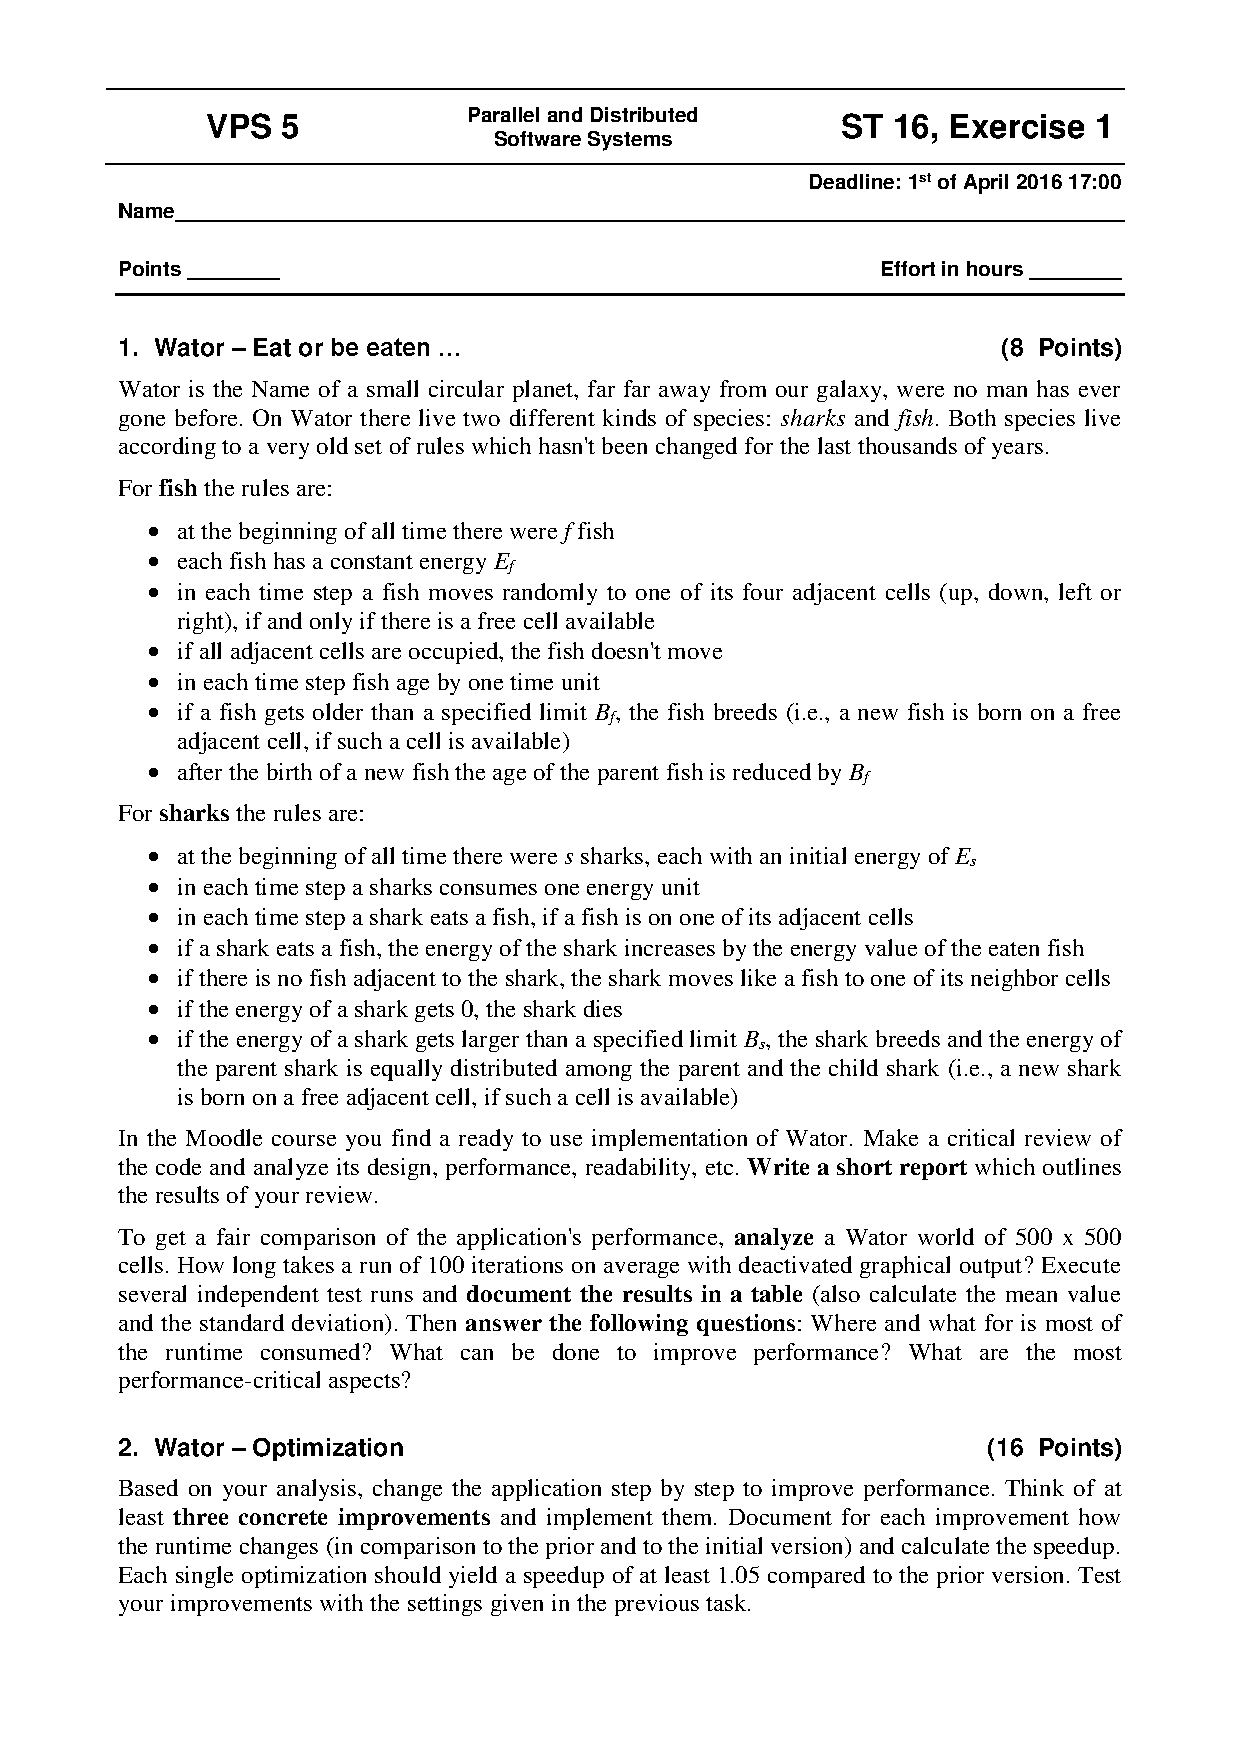
\includepdf[pages=-]{angabe.pdf}

\ihead{VPS SS 2016 - �bung 01}
\ifoot{Roman Lumetsberger}
\cfoot{1310307026}
\ofoot{Seite \pagemark}

\section{1. Wator � Eat or be eaten}
\subsection{Analyse}
Der Sourcecode ist grunds�tzlich gut dokumentiert und auch lesbar. 
Die Architektur der Anwendung loose gekoppelt und nachvollziehbar. Zur Implementierung gibt es zu erw�hnen, dass in der selben Methode oft auf die gleichen Feldelemente zugegriffen wird. Hier w�re es vielleicht
besser, wenn der Wert einmal zwischengespeichert werden w�rde, da sonst bei jedem Zugriff Laufzeit�berpr�fungen durchgef�hrt werden. 
Weiters f�llt auf, dass sehr viele Objekte der Klasse \texttt{Point} angelegt werden.
Zur Methode \texttt{GetNeighbors} gibt es zu erw�hnen, dass hier f�r alle vier Richtungen eigentlich der selbe Code verwendet wird und dieser vielleicht besser in eine Methode ausgelagert werden k�nnte (bringt 
warscheinlich keine Performancesteigerung aber der Code w�re besser lesbar).

\subsection{Where and what for is most of the runtime consumed?}
 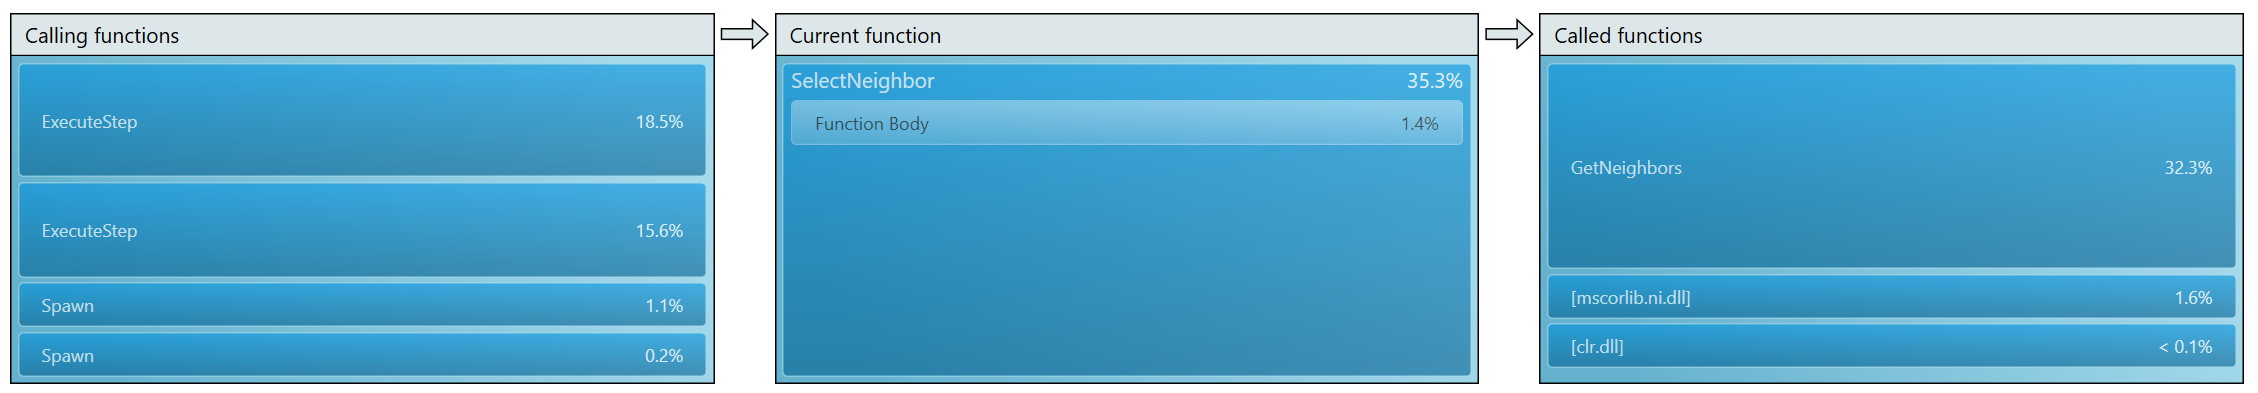
\includegraphics[width=400px]{images/profiling.png}

 Grunds�tzlich wird die meiste CPU-Zeit in der Methode \texttt{ExecuteStep} und in weiterer Folge dann in \texttt{GetNeighbors} verbraucht.
 Diese Methode ist f�r das Suchen der Nachbarn eines Feldes zust�ndig und wird daher sehr oft aufgerufen.
 Die Analsyse der Methode zeigt, dass sehr viele \texttt{Point} Objekte angelegt und dann sogar nochmals kopiert werden. Dadurch wird sehr viel CPU-Zeit verbraucht.

 Die Methode \texttt{RandomizeMatrix} ist eine weitere Methode die sehr viel CPU-Zeit ben�tigt. Diese ist f�r das Mischen der Durchlauf-Matrix zust�ndig.

\subsection{What can be done to improve performance?}
\begin{itemize}
	\item Umgang mit den Koordinaten in der Methode \texttt{GetNeighbors} optimieren, damit nicht mehr so viele Objekte angelegt werden m�ssen.
		\subitem Verwenden eines statischen Arrays.
		\subitem Kopieren des Arrays am Ende der Methode vermeiden.
	\item Umstellen der zweidimensionalen Felder auf eindimensionales Felder.
	\item �ndern \texttt{Moved} Eigenschaft um die zus�tzliche Schleife �ber alle Elemente zu sparen.
		\subitem Eine M�glichkeit w�re hier die Iterationsnummer zu verwenden. 
\end{itemize}
  
\section{2. Wator � Optimization }

	
\end{document}